\section{Wstęp}
Niniejszy projekt realizowany w ramach kursu "Rozproszone i obiektowe systemy baz danych" ma na celu zaprojektowanie oraz imlementację rozproszonej aplikacji, odpornej na awarię baz danych, pozwalającącej zarządzać stanem magazynowym oraz sprzedażą w sieci restauracji.

\subsection{Cele projektu}
Celem projektu jest stworzenie systemu pozwalającego zarządzać siecią restauracji. System pozwala na utworzenie nowej restauracji w bazie, utworzenie menu wspólnego dla całej sieci, zarządzania stanem magazynowym poszczególnych restauracji, sprzedaż produktów wpływająca na stan magazynowy. Dane o wszystkich restauracjach przechowywane są we wspólnej, centralnej bazie danych - wymaga ona maksymalnej dostępności oraz ochrony danych przed ich utratą. \\
Dostęp do systemu możliwy jest poprzez dowolną przeglądarkę internetową - użytkownik za pomocą interfejsu webowego posiada możliwość wykonywania operacji na bazie danych za pośrednictwem aplikacji serwerowej.


\begin{figure}[H]
	\centering
	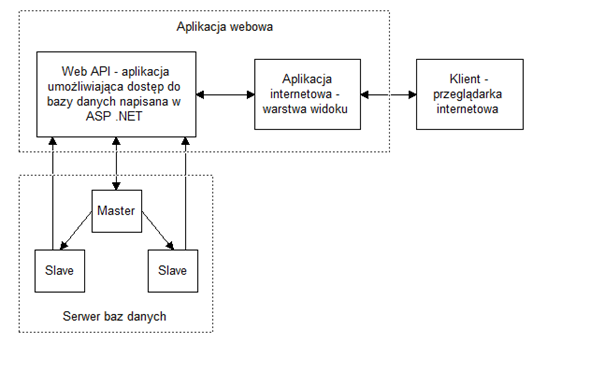
\includegraphics[width=\textwidth]{strukturaSystemu}
	\caption{Struktura systemu i schemat komunikacji}
\end{figure}


\subsection{Założenia projektowe}
Jako silnik bazy danych wybrany został system MongoDB ze względu na skalowalność, wydajność oraz architekturę zaprojektowaną z myślą o łatwej replikacji. Utworzone zostały trzy serwery bazy danych tworzące zestaw replik MongoDB. Webowa aplikacja kliencka został wykonana w oparciu o platformę ASP .NET MVC. 

